\section{Application 2: WikiCrime}

Collective intelligence is embedded in collaborative system. With the development of internet, collaborative system is becoming more and more popular. In the traditional Web (or Web 1.0), the differences between consumer and producer of information are pretty clear. Producers produce information and is then consumed by consumer. However, in the resent trend of the web (Web 2.0), there is no significant difference among information and producer. For example, many news on Twitter are now reported by individuals (user-generated contents) who are also users of Twitter. In a typical collaborative system, intelligence are distributed across the community and the outcome of collaborative system should collect all the intelligence and crystalize it to make it collective rather than collected.

Collaborative system has been widely used nowadays. One of the applications is to apply collaborative system to law enforcement domain. Current crime information system, in which the contents are provided by police and other government organization, has problems. For example, certain crimes are not notified to authorities, causing under-report phenomenon. Also, the public has no idea how the information are collected and generated, in another word, criminal information is opaque to the public.

In criminal information collaborative system, everyone is allowed to report crime to the system, which is coordinate by authorities, and the system employs an approach to gather all the related information and present it in a meaningful way. Then people can also benefit from it by checking the system to see if a place is safe or not. Nevertheless, there are some challenges in applying collective intelligence to crime information system. The major one is finding the equilibrium between people’s engagement and information credibility. On the one hand, anonymity make people prefer to report crime and provide information. On the other hand, the received information is less credible if the sources are unknown.

In the aforementioned context, WikiCrimes was developed. WikiCrimes is a Web 2.0 application that offers a collaborative environment for people to register and research criminal events. The interface, as shown in Figure~\ref{fig:WikiCrimeGUI}, is based on a map and users are able to manipulate the map. Other functions such as search criminal events based on location or time are provided as well. 

\begin{figure}[!h]
\centering
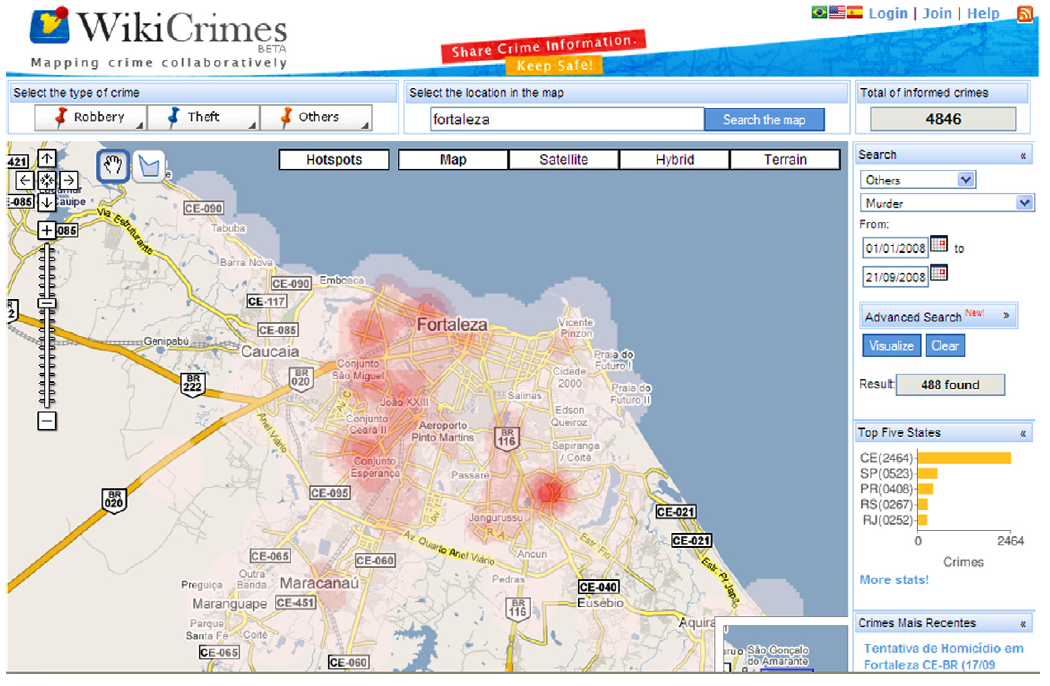
\includegraphics[width=0.9\columnwidth]{figure/wikicrime}
\caption{Graphical user interface for WikiCrime}
\label{fig:WikiCrimeGUI}
\end{figure}

WikiCrimes tries to provide a common interaction space among the public in which citizens are able to notify criminal facts as well as locations they happen. WikiCrimes are also driven by 1) providing more transparency and publicity to criminal information, 2) looking for means for citizen prevention and 3) reducing the phenomenon of under-reporting. WikiCrimes concentrate on how to guarantee the veracity and accuracy of information and how to take advantage of mining characterization of such crimes.

To implement a syetm that meet the goals mentioned before, WikiCrimes collaborative system is modeled as follows:

\centerline{WikiCrimes = {AS, AC, RE, OD, OS, OR, PI , N}}

Where, AS, agents playing system roles; Ac, agents playing context roles; RE, a set of external roles that are played by agents that interact with the system; OD, domain ontology (here identified as crime ontology); OS, system ontology; OR, reputation ontology; PI, Set of interaction protocols; N, set of norms represented as commitments among agent roles listed in RE. Among these, crime ontology and reputation ontology play significant roles since they are keys to how collective intelligence works in WikiCrimes.

Crime ontology contains mainly two kinds of entities, crime and report of crime. A crime has a type, a time, an address, and type of weapon used. The report of crime is more like meta-information, such as whether a crime is confirmed or is communicated to the police. By doing this, the outcomes of WikiCrime will be more convincing since not all crimes are equal so that they need to be associated with different weights according to the information of crime itself.

Reputation ontology is very important to WikiCrime. In a collaborative system, participants are equipped with diverse knowledge base. Some of them are capable of contributing more to the results while others might not be able to play a vital role. Besides, credibility of the information also depends on reputation of the information provider. Therefore, a reputation mechanism is necessary to distinguish participants with different intelligence.  Generally, the reputation score is calculated according to interaction activities and social evaluation. For instance, if a user reports crimes a lot and the reported crimes are always confirmed later, the user is considered to be a trustworthy one. Similarly, user’s performance is also evaluated by peers. In a nutshell, a well-designed reputation mechanism can help improve the results of a collaborative system, in this case, provide a more useful crime map.

Since data generated by WikiCrimes follows the same distribution pattern as one of official data (Ripley test), WikiCrimes has been proved to be an effective way of producing collective intelligence concerning crime events. But as explained in the original paper, WikiCrimes does not intend to replace official criminal information system. WikiCrimes aims to function as an auxiliary system of data collection that adds more quality to this process. For example, with the help of WikiCrimes, phenomenon of under-reporting can be discovered, criminal trend can be predicted and potential dangerous area can be identified.

Some improvements can be made as well. Nowadays almost everyone has a cellphone. With the popularity of smartphones, the process of reporting crimes and communicating with police is becoming more and more convenient and instant. Besides, not only people’s opinion can be collected, but also contents from newspapers and other media can be extracted to form crime-related information.

In a nutshell, applying collective intelligence to law enforcement domain is helpful. It offers a common interaction space among the public in general, so that each one of them is able to notify criminal facts. As a result. a collective crime report system can improve the quality of collected information and produce collective intelligence. 
